\documentclass[ignorenonframetext,]{beamer}
\usetheme{CambridgeUS}
\usecolortheme{sidebartab}
\setbeamertemplate{caption}[numbered]
\setbeamertemplate{caption label separator}{:}
\setbeamercolor{caption name}{fg=normal text.fg}
\usepackage{amssymb,amsmath}
\usepackage{ifxetex,ifluatex}
\usepackage{fixltx2e} % provides \textsubscript
\usepackage{lmodern}
\ifxetex
  \usepackage{fontspec,xltxtra,xunicode}
  \defaultfontfeatures{Mapping=tex-text,Scale=MatchLowercase}
  \newcommand{\euro}{€}
\else
  \ifluatex
    \usepackage{fontspec}
    \defaultfontfeatures{Mapping=tex-text,Scale=MatchLowercase}
    \newcommand{\euro}{€}
  \else
    \usepackage[T1]{fontenc}
    \usepackage[utf8]{inputenc}
      \fi
\fi
% use upquote if available, for straight quotes in verbatim environments
\IfFileExists{upquote.sty}{\usepackage{upquote}}{}
% use microtype if available
\IfFileExists{microtype.sty}{\usepackage{microtype}}{}
\usepackage{longtable,booktabs}
\usepackage{caption}
% These lines are needed to make table captions work with longtable:
\makeatletter
\def\fnum@table{\tablename~\thetable}
\makeatother
\usepackage{graphicx}
\makeatletter
\def\maxwidth{\ifdim\Gin@nat@width>\linewidth\linewidth\else\Gin@nat@width\fi}
\def\maxheight{\ifdim\Gin@nat@height>\textheight0.8\textheight\else\Gin@nat@height\fi}
\makeatother
% Scale images if necessary, so that they will not overflow the page
% margins by default, and it is still possible to overwrite the defaults
% using explicit options in \includegraphics[width, height, ...]{}
\setkeys{Gin}{width=\maxwidth,height=\maxheight,keepaspectratio}

% Comment these out if you don't want a slide with just the
% part/section/subsection/subsubsection title:
\AtBeginPart{
  \let\insertpartnumber\relax
  \let\partname\relax
  \frame{\partpage}
}
\AtBeginSection{
  \let\insertsectionnumber\relax
  \let\sectionname\relax
  \frame{\sectionpage}
}
\AtBeginSubsection{
  \let\insertsubsectionnumber\relax
  \let\subsectionname\relax
  \frame{\subsectionpage}
}

\setlength{\parindent}{0pt}
\setlength{\parskip}{6pt plus 2pt minus 1pt}
\setlength{\emergencystretch}{3em}  % prevent overfull lines
\setcounter{secnumdepth}{0}
\usepackage{multicol}
\usepackage{graphicx}

\title{Multivariable Regression in R}
\author{Phillip Ayieko}
\date{}

\begin{document}
\frame{\titlepage}

\begin{frame}{Principles of multivariable regression analysis}

\begin{itemize}
\itemsep1pt\parskip0pt\parsep0pt
\item
  MVA relate 2 or more independent variables to an outcome (through
  mathematical expression)
\end{itemize}

\[
Cholesterol \Longleftarrow age + exercise + diet
\]

\[
y_i = \beta_0 + \beta_1 x_i + \beta_2 x_i + \beta_3 x_i +  \epsilon_i
\]

\end{frame}

\begin{frame}{Main multivariable models in biostatistics}

\begin{itemize}
\itemsep1pt\parskip0pt\parsep0pt
\item
  Generalized linear models
\item
  A generalized linear model is made up of a linear predictor = relates
  mean to predictors
\item
  and two functions:
\item
  a link function (transform done on Y) = relates means of observations
  to predictors \[
  Cholesterol \Longleftarrow age + exercise + diet
  \]
\item
  a variance function (the distribution) = relates the means to the
  variances
\end{itemize}

\end{frame}

\begin{frame}{Main multivariable models in biostatistics}

\begin{longtable}[c]{@{}ll@{}}
\toprule
Type of MVA regression & Typical Use\tabularnewline
\midrule
\endhead
Multiple (general) linear & Predicting a quantitative response variable
from 2 or more explanatory variables\tabularnewline
Logistic & Predicting a categorical response variable from 2 or more
explanatory variables\tabularnewline
Poisson & Predicting a response variable representing counts from 2 or
more explanatory variables\tabularnewline
Cox proportional hazards & Predicting time to event (death, failure,
relapse) from 2 or more explanatory variables\tabularnewline
Time series & Modelling time series data with correlated
errors\tabularnewline
Discriminant function analysis & Predicting a group to which subjects
belong (commonly use a score to classify obs into one of the categorical
groups) -,c.f Logistic regression\tabularnewline
\bottomrule
\end{longtable}

\end{frame}

\begin{frame}{``Multivariate'' or ``Multivariable'' analysis?}

\begin{itemize}
\itemsep1pt\parskip0pt\parsep0pt
\item
  Often used interchangeably, but:
\item
  Multivariable - single outcome
\item
  Multivariable - multiple outcomes e.g.~factor analysis
\end{itemize}

\end{frame}

\begin{frame}{Purposes of Multivariable Analysis}

\begin{itemize}
\itemsep1pt\parskip0pt\parsep0pt
\item
  Bivariate confirmation
\item
  Multivariable Confirmation
\item
  Screening
\item
  Creating Risk Scores
\item
  Quantifying Risk of Individual Variables
\end{itemize}

\end{frame}

\begin{frame}{Common problems with MVA}

\begin{itemize}
\itemsep1pt\parskip0pt\parsep0pt
\item
  Over-fitting or under-fitting
\item
  Nonconformity to a Linear Gradient
\item
  Violation of proportional hazards assumption
\item
  No report of tests for interaction
\item
  Unspecified coding of variables
\item
  Unspecified selection of variables
\item
  Collinearity of variables
\item
  Influential observations
\item
  Model validation
\end{itemize}

\end{frame}

\begin{frame}{Over-fitting or under-fitting}

\[
Death \Longleftarrow smoking
\]

\(\circ Non-smoker \bullet smoker\)

\end{frame}

\begin{frame}{Over-fitting or under-fitting}

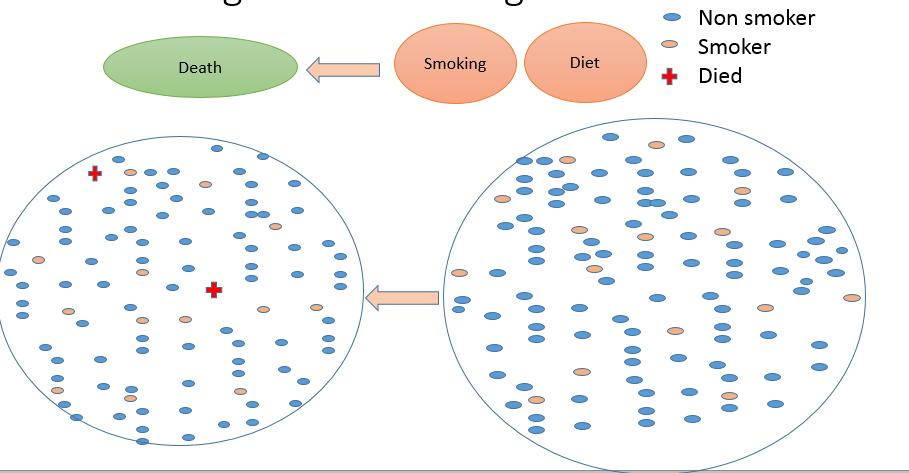
\includegraphics{overfit.png}

\end{frame}

\begin{frame}{Implications}

\begin{longtable}[c]{@{}ll@{}}
\toprule
& Impact\tabularnewline
\midrule
\endhead
Overfiting & Unreliable risk estimates/ low precision\tabularnewline
& Spurious associations\tabularnewline
Under-fitting (variable omission/ underpowered analysis) & Predicting a
response variable representing counts from 2 or more explanatory
variables\tabularnewline
& Misleading results\tabularnewline
\bottomrule
\end{longtable}

\end{frame}

\begin{frame}{Violation of PH assumption (Cox regression)}

\begin{itemize}
\item
  Hazard ratio - does not depend on time (on covariates only)
\item
  Methods for verification
\item
  Plot of `cumulative baseline hazard estimates on a log-scale': Curves
  on the plot should be parallel with distance that is constant over
  time
\item
  Survival curves: if PH assumption is met survival curve of one group
  will not cross the survival curve of other group
\end{itemize}

\end{frame}

\begin{frame}{PH assumption}

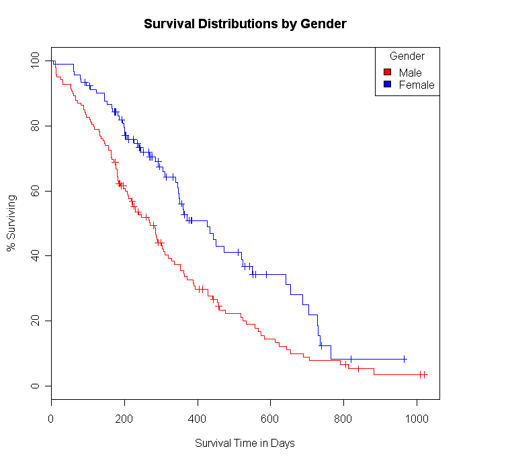
\includegraphics{gender.png}

\end{frame}

\begin{frame}{Checking PH assumption in `R'}

\end{frame}

\begin{frame}{No report of tests for interaction}

\begin{itemize}
\itemsep1pt\parskip0pt\parsep0pt
\item
  To be covered in the next session
\end{itemize}

\end{frame}

\begin{frame}{Unspecified coding}

\begin{itemize}
\itemsep1pt\parskip0pt\parsep0pt
\item
  readers should always be notified of how the coding was used in a
  multivariable analysis:
\item
  Marginal (binary variable -1/+1) v.s. partial (binary variable 0/1)
  methods
\item
  Ordinal variable coding = could use ``dummy'' variable or integer
  values
\item
  Regression coefficients reported without concomitant citation of unit
  of coding e.g.~single coefficient for age - could mean continuous
  variable or a dichotomous variable (\textless{}5/ above 5 years)
\end{itemize}

\end{frame}

\begin{frame}{Unspecified Selection of Variables}

\begin{itemize}
\itemsep1pt\parskip0pt\parsep0pt
\item
  Strategies of variable selection for MVA

  \begin{itemize}
  \itemsep1pt\parskip0pt\parsep0pt
  \item
    Previous research
  \item
    Clinical experience
  \item
    Automated algorithms - esp. prognostic studies
  \end{itemize}
\item
  Final model depends on the chosen selectin process
\end{itemize}

\end{frame}

\begin{frame}{Summary}

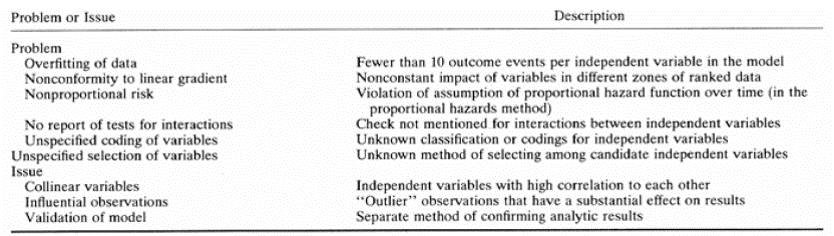
\includegraphics{summary.png}

\end{frame}

\begin{frame}{Principle MV models in `R'}

\begin{itemize}
\itemsep1pt\parskip0pt\parsep0pt
\item
  multivariable\_reg\_practical.pdf
\end{itemize}

\end{frame}

\begin{frame}{Introduction Interaction \& Effect Modification}

Introduction Interaction \& Effect Modification

\end{frame}

\begin{frame}{Interaction/ effect modification}

\begin{itemize}
\itemsep1pt\parskip0pt\parsep0pt
\item
  Most of the outcomes (events) are determined (influenced) by more than
  one factor (e.g.~body weight.)
\end{itemize}

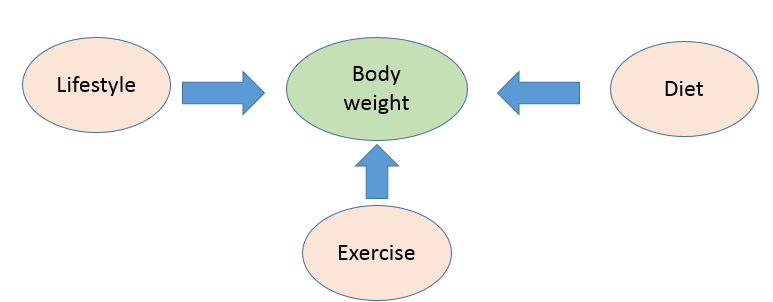
\includegraphics{lifestyle.png}

\end{frame}

\begin{frame}{Interaction/ effect modification}

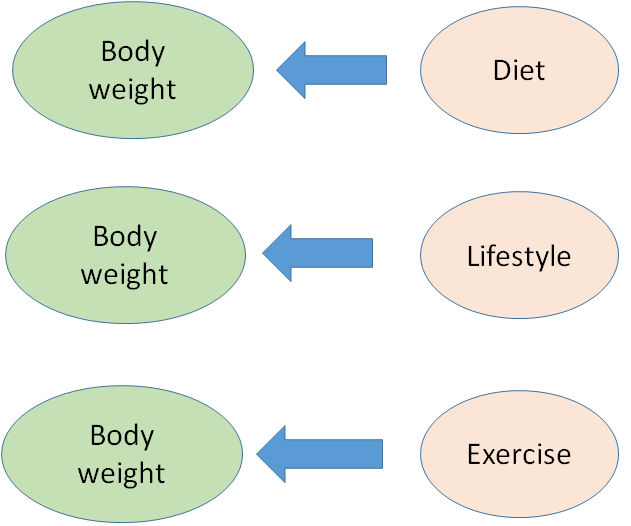
\includegraphics{lifestyle2.png}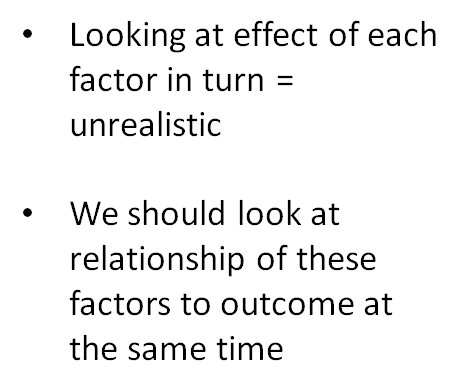
\includegraphics{lifestyle3.png}

\end{frame}

\begin{frame}{Interaction/ effect modification}

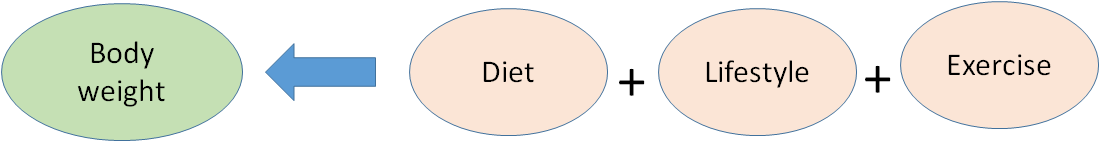
\includegraphics{lifestyle4.png}

\begin{itemize}
\itemsep1pt\parskip0pt\parsep0pt
\item
  When we look at the relation of these factors (explanatory variables)
  to the outcome at the same time, \ldots{}.

  \begin{itemize}
  \itemsep1pt\parskip0pt\parsep0pt
  \item
    We will obtain the ``independent effect'' of explanatory variables
    to outcome.
  \item
    We can also study the ``interaction'' (IA) between independent
    variables (Synergistic/Antagonistic IA)
  \end{itemize}
\end{itemize}

\end{frame}

\begin{frame}{Interaction}

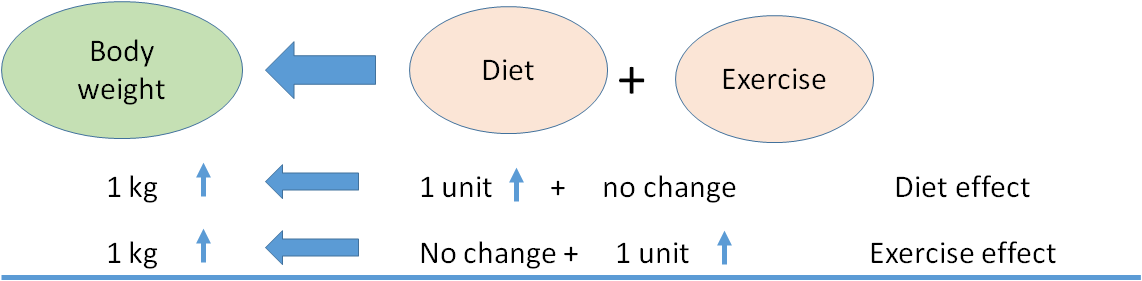
\includegraphics{lifestyle5.png}

\end{frame}

\begin{frame}{Interaction}

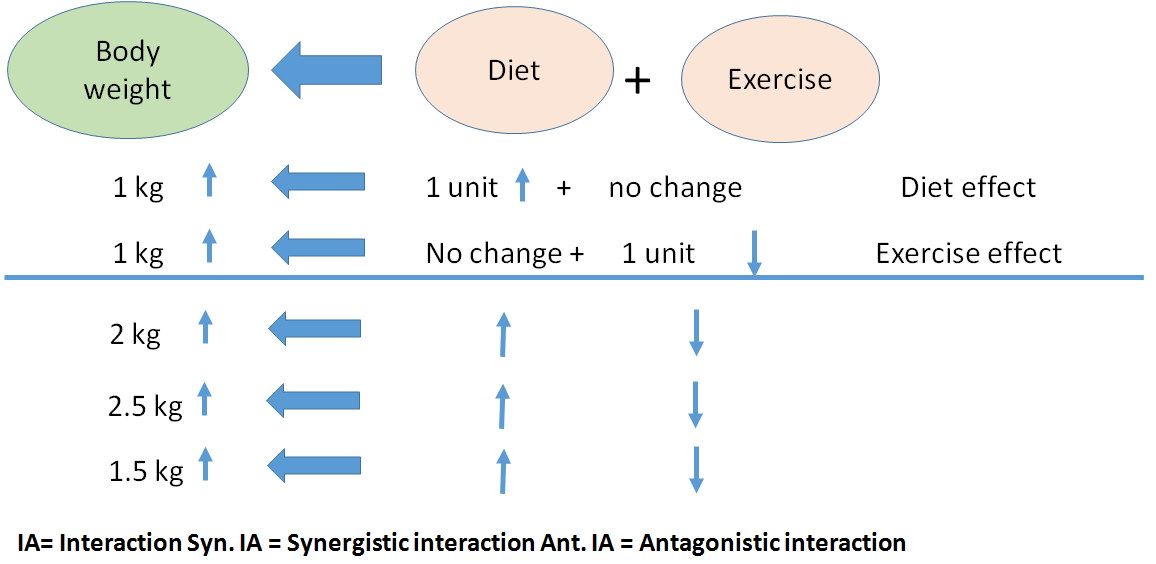
\includegraphics{lifestyle6.png}

\end{frame}

\begin{frame}{Detection/interpretation of interaction \& effect
modification}

\begin{itemize}
\itemsep1pt\parskip0pt\parsep0pt
\item
  An interaction occurs when the product of two predictor variables is
  also a significant predictor (i.e.~in addition to the predictor
  variables themselves)
\item
  Create an interaction term
\item
  Perform likelihood ratio test (LRT)
\end{itemize}

\end{frame}

\begin{frame}{Testing for interaction in `R'}

\begin{itemize}
\itemsep1pt\parskip0pt\parsep0pt
\item
  interaction practical.pdf
\end{itemize}

\end{frame}

\begin{frame}{Confounding and stratification}

Confounding and stratification

\end{frame}

\begin{frame}{Exposures and outcomes}

In an epidemiological study there is: a. the outcome of interest b. the
primary exposure (or risk factor) of interest c. other exposures that
may influence the outcome (potential confounders)

\end{frame}

\begin{frame}{Exposures and outcomes}

\begin{itemize}
\itemsep1pt\parskip0pt\parsep0pt
\item
  You will need to measure more than one exposure
\end{itemize}

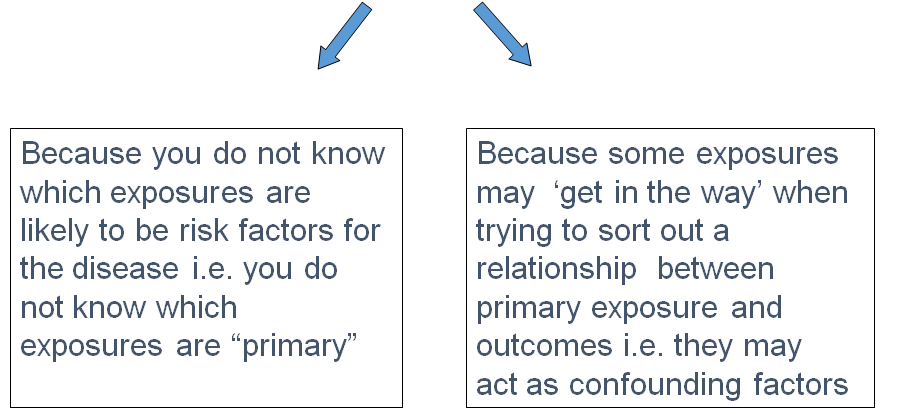
\includegraphics{lifestyle7.png}

\end{frame}

\begin{frame}{Question: Is alcohol consumption during pregnancy
associated with increased risk of low birthweight ?}

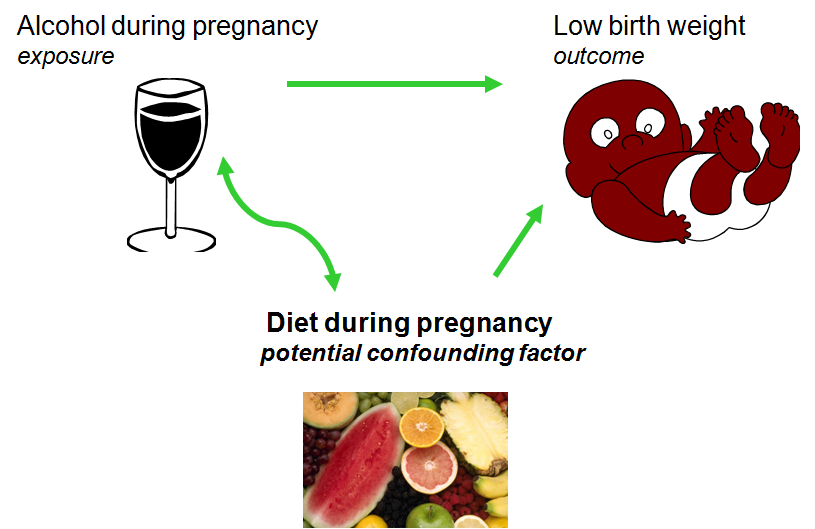
\includegraphics{lifestyle8.png}

\end{frame}

\begin{frame}{Confounding is about}

\textbf{ALTERNATIVE EXPLANATIONS FOR AN EFFECT SEEN} - when an
association between the Exposure under investigation and Outcome is
``mixed up'' with the effect of another exposure or exposures - when the
effects of the two exposures have not been considered separately
\(OR = 1.40\) reflects true association.

\end{frame}

\begin{frame}{Confounding: Definition: for a factor to be regarded as a
confounder the rules are:}

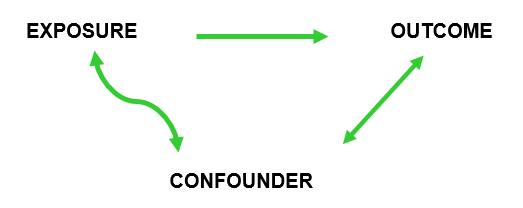
\includegraphics{exposure.png}

\begin{enumerate}
\def\labelenumi{\arabic{enumi}.}
\itemsep1pt\parskip0pt\parsep0pt
\item
  The factor must be associated with the exposure being investigated
\item
  The factor must be independently associated with the disease being
  investigated.
\item
  The confounder is not on the causal pathway.
\end{enumerate}

\end{frame}

\begin{frame}{How to deal with confounding}

\begin{itemize}
\itemsep1pt\parskip0pt\parsep0pt
\item
  Need to display the data separately for each level of the confounding
  factor
\item
  Then examine the measures of effect within eachlevel (or strata)
\item
  If they different from the ``crude'' measure of effect, but similar to
  each other, this is evidence of confounding \emph{BUT no test for
  confounding.}
\end{itemize}

\end{frame}

\begin{frame}{Example: Case-control study of coffee comsumption and
cancer of the pancreas}

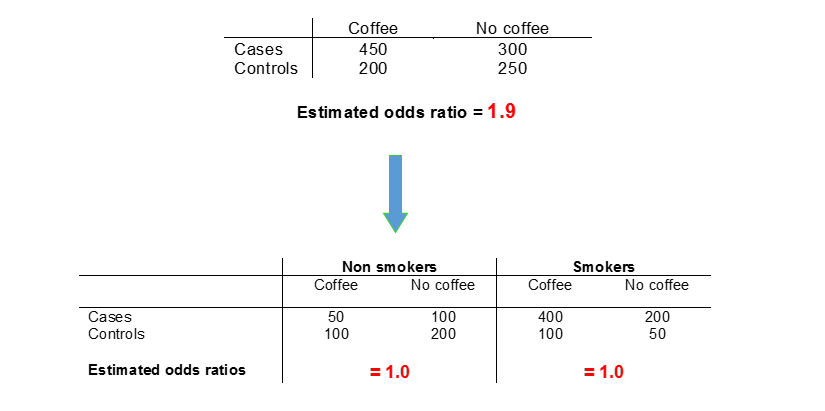
\includegraphics{coffee_cancer.png}

\end{frame}

\begin{frame}

\begin{itemize}
\itemsep1pt\parskip0pt\parsep0pt
\item
  We have shown that the ``stratified'' measure of effect (in this case
  odds ratios) are different from the ``crude'' measure of effect, but
  similar to each other
\item
  Thus we have evidence that Smoking was acting as a confounding factor
\end{itemize}

\textbf{Question: What is the odds ratio for the effect of Smoking on
the risk of cancer of the pancreas?}

Use data from table below:

\begin{longtable}[c]{@{}lllll@{}}
\toprule
& Non Smoker & & Smoker &\tabularnewline
\midrule
\endhead
& Coffee & No Cofee & Coffee & No coffee\tabularnewline
cases & 50 & 100 & 400 & 200\tabularnewline
control & 100 & 200 & 100 & 50\tabularnewline
& & & &\tabularnewline
\bottomrule
\end{longtable}

\end{frame}

\begin{frame}

\(Answer= (600 * 300 ) / (150* 150) = 8\)

\end{frame}

\begin{frame}

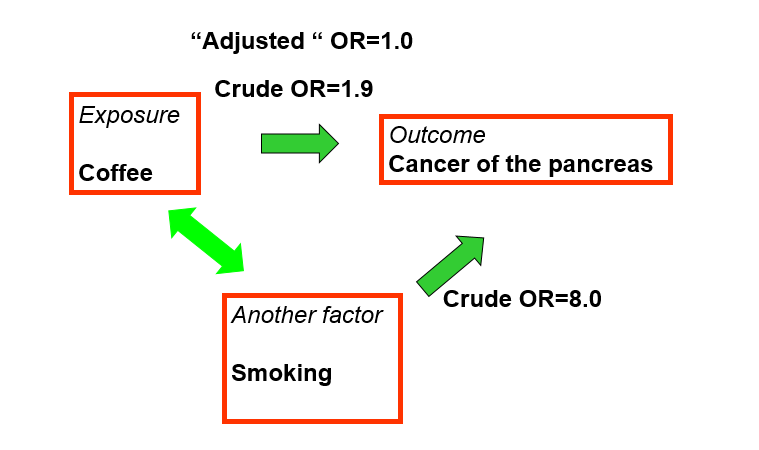
\includegraphics{odds_adjusted.png}

\end{frame}

\begin{frame}

\begin{itemize}
\itemsep1pt\parskip0pt\parsep0pt
\item
  we investigate the control data further, we can see that the
  confounding factor is associated with the exposure under
  investigation:
\end{itemize}

\begin{longtable}[c]{@{}lll@{}}
\toprule
& Coffee & No Coffee\tabularnewline
\midrule
\endhead
Smoker & 100 (50\%) & 50(20\%)\tabularnewline
Non Smoker & 100 & 200\tabularnewline
------------ & ----------- & -----------\tabularnewline
& 200(100\%) & 250\tabularnewline
\bottomrule
\end{longtable}

\begin{itemize}
\itemsep1pt\parskip0pt\parsep0pt
\item
  1 in 2 coffee drinkers are smokers
\item
  1 in 5 non-coffee drinkers are smokers
\end{itemize}

\end{frame}

\begin{frame}

\begin{itemize}
\itemsep1pt\parskip0pt\parsep0pt
\item
  This example demonstrated complete confounding where \textbf{ALL} the
  association between coffee drinking and cancer of the pancreas could
  be``explained'' by smoking

  \begin{itemize}
  \itemsep1pt\parskip0pt\parsep0pt
  \item
    \textbf{i.e: OR of 1.9 was reduced to 1.0}
  \end{itemize}
\item
  Other examples may give PARTIAL confounding

  \begin{itemize}
  \itemsep1pt\parskip0pt\parsep0pt
  \item
    \textbf{i.e: Rate Ratio of 2.5 was reduced to 2.0}
  \end{itemize}
\item
  But remember that measures of effect can go UP as well as DOWN :
  \textbf{NEGATIVE} confounding
\end{itemize}

\end{frame}

\begin{frame}{SECTION II}

SECTION II

\end{frame}

\begin{frame}{How to deal with confounding}

\begin{itemize}
\itemsep1pt\parskip0pt\parsep0pt
\item
  At the Design Stage

  \begin{itemize}
  \itemsep1pt\parskip0pt\parsep0pt
  \item
    Randomisation
  \item
    Restriction
  \item
    Matching
  \end{itemize}
\item
  At the Analysis Stage

  \begin{itemize}
  \itemsep1pt\parskip0pt\parsep0pt
  \item
    Stratification
  \item
    Standardisation
  \item
    Statistical modelling
  \item
    eg logistic regression
  \end{itemize}
\end{itemize}

But need to have collected the data\ldots{}.

\end{frame}

\begin{frame}{FURTHER ANALYSIS OF 2X2 TABLES}

\textbf{Mantel-Haenszel methods:} - 1.Mantel-Haenszel technique to
obtain ORMH adjusted for confounding factor. - 2. Mantel-Haenszel
\(\chi^2\) to test whether adjusted \(OR = 1.\)

\#\# Case-control study of coffee drinking and pancreatic cancer

\begin{longtable}[c]{@{}llll@{}}
\toprule
& & casse & control\tabularnewline
\midrule
\endhead
coffee & yes & 450 & 440\tabularnewline
drinking & no & 300 & 410\tabularnewline
& total & 750 & 850\tabularnewline
\bottomrule
\end{longtable}

\[
Crude OR = ad / bc = 450x410 / 440x300 = 1.40.
\]

\begin{itemize}
\itemsep1pt\parskip0pt\parsep0pt
\item
  Suggests risk of pancreatic cancer associated with coffee drinking.
\end{itemize}

\end{frame}

\begin{frame}

\begin{itemize}
\item
  \(OR=1.40\)
\item
  Possible explanations:

  \begin{itemize}
  \itemsep1pt\parskip0pt\parsep0pt
  \item
    Chance: -\(\chi^2 (O-E) = 10.62, p=0.001 \Rightarrow\) chance is
    unlikely.
  \item
    Bias:
  \item
    OR = 1.40 does not represent the true OR.
  \item
    Confounding:
  \item
    OR = 1.40, but due to effect of other variable.
  \item
    Causation:
  \item
    OR = 1.40 reflects true association.
  \end{itemize}
\end{itemize}

\end{frame}

\begin{frame}{Look within stratum of confounding variable}

\begin{longtable}[c]{@{}lllllll@{}}
\toprule
& & smokers & & & non smoker &\tabularnewline
\midrule
\endhead
& & case & control & & case & control\tabularnewline
coffee & yes & 400 & 340 & & 50 & 100\tabularnewline
& no & 200 & 190 & & 100 & 220\tabularnewline
& & 600 & 530 & & 150 & 320\tabularnewline
\bottomrule
\end{longtable}

\begin{itemize}
\itemsep1pt\parskip0pt\parsep0pt
\item
  Is smoking associated with increased risk of pancreatic cancer?
\item
  600 (80\%) of the 750 cases are smokers
\item
  530 (62\%) of the 850 controls are smokers
\end{itemize}

\end{frame}

\begin{frame}{Look within stratum of confounding variable}

\begin{longtable}[c]{@{}lllllll@{}}
\toprule
& & smokers & & & non smoker &\tabularnewline
\midrule
\endhead
& & case & control & & case & control\tabularnewline
coffee & yes & 400 & 340 & & 50 & 100\tabularnewline
& no & 200 & 190 & & 100 & 220\tabularnewline
& & 600 & 530 & & 150 & 320\tabularnewline
\bottomrule
\end{longtable}

\begin{itemize}
\itemsep1pt\parskip0pt\parsep0pt
\item
  Are coffee drinkers more likely to smoke?
\item
  Among controls.
\item
  340 of the 440 coffee drinkers are smokers (77\%)
\item
  190 of the 410 non-coffee drinkers are smokers (46\%)
\end{itemize}

\end{frame}

\end{document}
